%%%%%%%%%%%%%%%%%%%%%%%%%%%%%%%%%%%%%%%%%%% 
% Marco Caserta (c) 2020
% marco dot caserta at ie dot edu
%%%%%%%%%%%%%%%%%%%%%%%%%%%%%%%%%%%%%%%%%%% 
\documentclass[12pt]{article}
\usepackage{palatino}
\linespread{1.07}        % Palatino needs more leading
\usepackage[margin=0.75in]{geometry}
\usepackage{amsmath,amsfonts,amsthm,amssymb}
\usepackage{algorithm,algorithmic}
\usepackage{epstopdf}
\usepackage{eurosym}
\usepackage{lastpage}
\usepackage{fancyhdr}
\usepackage{floatflt,graphicx}
\usepackage{multirow}
\usepackage{lettrine}
\usepackage{pgfplots}
\usepackage{url}
\renewcommand{\LettrineFontHook}{\color[gray]{0.5}}

\pgfmathdeclarefunction{gauss}{2}{%
  \pgfmathparse{1/(#2*sqrt(2*pi))*exp(-((x-#1)^2)/(2*#2^2))}%
}

% \oddsidemargin -1.0cm \evensidemargin 0.0cm \textwidth 18cm \textheight 20cm \headsep 20pt
\headheight 70pt \topmargin -1cm 
\textheight 20.5cm
% \footsep 10pt

% \fboxsep=1cm
\title{Orienteering - The Unesco Challenge}
\author{Marco Caserta}
\date{}

\begin{document}

\maketitle

\section{Problem Description}

The Unesco Challenge is aimed at finding a maximum prize route across a set
of sites without exceeding a maximum travelling time. In addition, a few side
constraints are to be considered (e.g., balance of the solution in terms of
type of sites visited) and by the fact that the prize associated to a site
depends on some of the other sites included in the route.

A mathematical model for the problem can be sketched as follows. Let us define
the following sets:
\begin{itemize}
\item $P$: set of candidate places, or sites ($j=1,\dots,|P|$). We indicate with $P' = P
\cup\left\{ 0 \right\}$ the set which includes home, labelled as site
$0$;
\item $S$: set of countries ($k=1,\dots,|S|$);
\item $S_k$ : set of sites in country $k$;
\item $D$ : set of endangered sites;
\item $C$, $N$, and $M$: set of cultural, natural, and mixed places.
\end{itemize}
In addition, we define the following variables:
\begin{itemize}
\item $x_{ij}$ takes value $1$ if site $j$ is visited after site $i$ and
$0$ otherwise, for $i,j \in P'$;
\item $y_j$ takes value $1$ if site $j$ is visited, and $0$ otherwise, for $j
\in P$;
\item $z_k$ takes value $1$ if country $k$ is visited and $0$ otherwise, with
$k \in S$.
\end{itemize}
Therefore, the problem can be formulated as:
\begin{align}
 (OP): \max & \sum_{j\in P} y_j + \sum_{k \in S} 2\times z_k + \sum_{j \in D}3\times
  y_i\\
  \mbox{s.t.} \;\;\;\;   &  
    \sum_{i\in P'} \sum_{j\in P'} t_{ij}x_{ij} \leq B
    \label{eq:budget}\\
    & \sum_{i\in P} x_{ij} \geq y_j, \quad j \in P \label{eq:selected}\\
    & \sum_{j\in S_k} y_{j} \geq z_k, \quad k \in S\label{eq:country}\\
    & | \sum_{j\in C} y_j - \sum_{j \in N} y_j | \leq \sum_{j\in M}
    y_j + 1 \label{eq:balance}\\
    & \text{subtour elimination constraints}\\
    & x_{ij} \in \left\{ 0,1 \right\}, \quad i,j \in P' \\
    & y_{j} \in \left\{ 0,1 \right\}, \quad j \in P \\
    & z_{k} \in \left\{ 0,1 \right\}, \quad k \in S
\end{align}
where $t_{ij}$ indicates the travel time between site $i$ and site $j$, and $B$
is the available travel time.

The objective function maximizes the overall score of a solution, given by the
weighted sum of the number of sites, the number of countries, and the number of
visited endangered sites. Constraint \eqref{eq:budget} ensures that the
maximum traveling time is not exceeded; constraints \eqref{eq:selected} ensure
that a site is accounted for only if it is a destination of another point;
constaints \eqref{eq:country} guarantee that the country variable takes up
a value of 1 only if at least one site of that country has been selected;
finally, constraint \eqref{eq:balance} captures the satisfaction of the following
property: an equal number of sites of type C and type N are visited, where
sites of type M can be classified as needed. More precisely, in order not to
restrict the domain of the solutions to routes with an even number of sites, the
constraint enforces that the maximum difference between the number of sites of
type C and N (after adjusting the classification of sites of type M) is at most
1. Later on, we will illustrate how this can easily be changed if an even
number of sites must be ensured. The last three constraints define the nature
of the variables, i.e., this model is a 0-1 (binary) program, since all the
variables are binary. Finally, in order to ensure a valid tour (at
least, in the TSP sense), subtour elimination constraints should be added here
(e.g., the Miller-Tucker-Zemlin subtour elimination constraints.)

Two hypotheses, not explicitly mentioned in the assignment, have been
introduced here:
\begin{itemize}
\item The first one is that constraint \eqref{eq:balance} is correct. The
constraint presented above is a more general version of the requirement, in the
sense that it allows a maximum inbalance of one site between sites of type C
and N. That is, it does not restrict the solution space to routes with an even
number of sites.  However, both the model and the associated code can easily be
modified by removing the ``+1'' from the constraint.
\item Subtours are not allowed, in the spirit of the Traveling Salesman
Problem.
\end{itemize}

\section{Solution Strategy and Algorithm}

The model presented in the previous section resembles a well-known problem
from the literature, the Orienteering problem, in which one has to select nodes
from a graph to maximize the prize collected at each node without exceeding a
budget (typically, a distance.) The problem studied here has the added
complication provided by the balance constraint \eqref{eq:balance}. Since the
Orienteering problem is known to be $\mathcal{NP}$-Hard, we assume that (OP) is
also $\mathcal{NP}$-Hard. This claim would require a rigorous prove (by
reduction) but it seems reasonable at this point.

In addition, given that the objective function coefficient of many of the binary
variables is the same, the reduced costs in a linear relaxation would tend to
be quite similar and, therefore, not too informatives in terms of dominance
across variables. It is reasonable to expect that the linear relaxation of
(OP) will produce quite loose bounds. In light of these considerations, we did
not attempt to use a mathematical programming-based technique to solve the
problem and we decided to resort to (meta)-heuristic schemes.

The algorithm implemented for (OP) is based on a simple implementation of a
metaheuristic known as
Iterative Local Search (ILS). The ILS has been successfully
employed in the context of the Orienteering problem. The basic structure of the
algorithm is provided below in Algorithm 1.

\floatname{algorithm}{Algorithm}
\begin{algorithm}
  \caption{: \texttt{ILS()} } \label{algo:generalCM}
  \begin{algorithmic}[1]
    \REQUIRE problem OP, stopping criteria, coordinates of home site
    \ENSURE best feasible route $\textbf{r} = \left(\mathbf{x}, \mathbf{y},
    \mathbf{z}\right)$
    \STATE $k = 0$ (iterations counter)
    \STATE relax constraint \eqref{eq:balance} and build incumbent solution
    $\textbf{r}^I$ with \texttt{insertion\_heuristic()}
    \WHILE{not stopping criteria}
    \STATE $k \leftarrow k+1$ (iteration counter)
    \STATE \texttt{no\_improv} $=0$ (nr.  iterations without improvements)
    \STATE $\textbf{r}^I \leftarrow$ \texttt{repair\_heuristic($\textbf{r}^I$)} to re-introduce constraint \eqref{eq:balance}
    \STATE \texttt{stop = false}
    \WHILE{\texttt{!stop}}
    \STATE relax \eqref{eq:balance} and $\textbf{r} \leftarrow$ \texttt{2-Opt($\textbf{r}^I$)} heuristic to repaired incumbent
    \STATE $\textbf{r} \leftarrow$ \texttt{repair\_heuristic($\textbf{r}$)} to re-introduce constraint \eqref{eq:balance} 
    \IF{$\textbf{r}$ is an improving solution}
    \STATE $\textbf{r}^I \leftarrow \textbf{r}$
    \STATE \texttt{no\_improv} $=0$
    \ELSE
    \STATE increament \texttt{no\_improv} by one
    \STATE if max number of iterations without improvements has been reached,
    \texttt{stop = true}
    \ENDIF
    \ENDWHILE
    \STATE update best route $\textbf{r}^*$ if needed
    \STATE $\textbf{r}^I \leftarrow$
    \texttt{random\_perturbation($\textbf{r}^I$)} heuristic
    (remove \% of sites in $\textbf{r}^I$)
    \ENDWHILE
  \end{algorithmic}
\end{algorithm}

The algorithm \texttt{ILS()} is therefore based on four heuristics, briefly
described below:
\begin{itemize}
\item \texttt{insertion\_heuristic()}: Starting from a solution that only
contains the home site, we add, in a greedy fashion, sites to the current
solution, as long as a site can be added without violating the budget
constraint \eqref{eq:budget}. In this phase, the balance constraint
\eqref{eq:balance} is ignored. Therefore, at the end of this phase, the
solution need not be feasible with respect to the balance constraint. Details
on the greedy score are presented in the documentation of the code accompanying
this document (under \texttt{docs/HTML}.)
\item \texttt{repair\_heuristic()}: Transforms the incumbent solution into a
balanced one, enforcing the satisfaction of constraint \eqref{eq:balance}, in
two different ways:
\begin{itemize}
\item swapping: remove from the current solution one site belonging to the
class in excess (C or N), and add from the available solution a site of the
opposite class. The swap is selected in such a way that the change in the
objective function is maximized, without violating the time limit constaint;
\item random removal: if a feasible swap is not found and yet the solution does
not satisfy constaint \eqref{eq:balance}, a site belonging to the largest class
is randomly selected and removed from the current solution.
\end{itemize}
This two-step approach is iteratively applied until a feasible solution is
reached.
\item \texttt{2-Opt()}: A classical 2-opt move is applied, in which a site that
is currently in the solution is swapped with one not in the solution, with the
aim of maximizing the increase in objective function value. This heuristic
operates on a relaxed version of (OP), in which the balance constraint is
removed. Therefore, after the 2-Opt scheme, the heuristic scheme must be
applied again.
\end{itemize}

The four-heuristics scheme benefits from multiple restarts, due to the random
mechanisms of \texttt{random\_perturbation()} and
\texttt{repair\_heuristic()}. Therefore, as long as a predefined number of
iterations has not been reached, we take the current solution and randomly
remove up to a $\gamma\%$ of sites from the current route. We thus obtain a new
incumbent, and we restart the cycle.

The stopping criteria are defined by two conditions, and we stop whenever the
first is reached: either (i) a maximum number of iterations without improvements has
been reached or (ii) a total maximum number of iterations has been completed.

\section{Data Structure and Implementation Issues}

A full description of the project structure is provided under the
\texttt{docs} folder of the project. The file \texttt{index.html} under the
\texttt{HTML} folder provides an overview of the organization of the project.
Details about the implementations are thereby presented.

With respect to the implementation of algorithm \texttt{ILS()}, we defined the
following classes:
\begin{itemize}
\item \texttt{Orienteering}: The main class, implementing all the heuristics of
the ILS cycle and
containing the basic data structure. To import the instance data, we created a
\texttt{DataFrame} as a list of \texttt{Records}. Each record contains all the
information available on a site (id, name, coordinates, country, etc.)
\item \texttt{Move}: This class implements the different moves carried out by
the heuristics, namely:
\begin{itemize}
\item the insertion move of the greedy insertion heuristic;
\item the removal-and-insertion move of the repair heuristic;
\item the swap move of the 2-Opt heuristic;
\item the random removal of sites of the random perturbation heuristic.
\end{itemize}
\item \texttt{Solution}: This class contains the data of a solution, i.e., the
\texttt{inSet} (the set of sites in the current solution), \texttt{outSet}
(the set of sites not in the current solution), the objective function value of
the current solution \texttt{Z}, the total travel time \texttt{time}, the set
of visited countries \texttt{countrySet}, etc. In addition, this class defines
the actual updates on to the solution, i.e., how a new node is added to the
route, how the 2-Opt swap is carried out.
\end{itemize}

We also defined auxiliary classes to parse the command line, as described in
the project documentation, under the folder \texttt{docs}.

\paragraph{Observations.} Since the algorithm is based on the exploration of
multiple neighbhorhoods, we placed special care on the solution evaluation
functions. More specifically, every time a new solution in a neighborhood is
reached, such routes must be evaluated in terms of (i) objective function
value, and (ii) time constraint. Rather than recomputing the objective function
value and the time associated to a solution, we keep track of the variation of
these two scores generated by each move. Therefore, the full computation of the
value of the objective function and of the travel time is no longer needed, if
a proper accounting of the moves is carried out throughout the local search.

Figure~\ref{fig:example} illustrates a solution obtained using as home point
the offices of the company in London. The solution is composed of 49 sites, 15 of these
endengered sites, and 38 different countries. The objective function value is
170 and the total travel time is 30228 minutes (ouf of an available total of
30240 minutes), which corresponds to a trip of 16784 km. It is worth
remembering that the travel time is the sum of two terms, the actual travel
time from site to site and the visiting time (6 hours) of each place visited.
On the other hand, the travel distance, in km, corresponds to the sum of the
distances from site to site. This explains the discrepancy between the two
numbers.

\begin{figure}[htb]
\centering
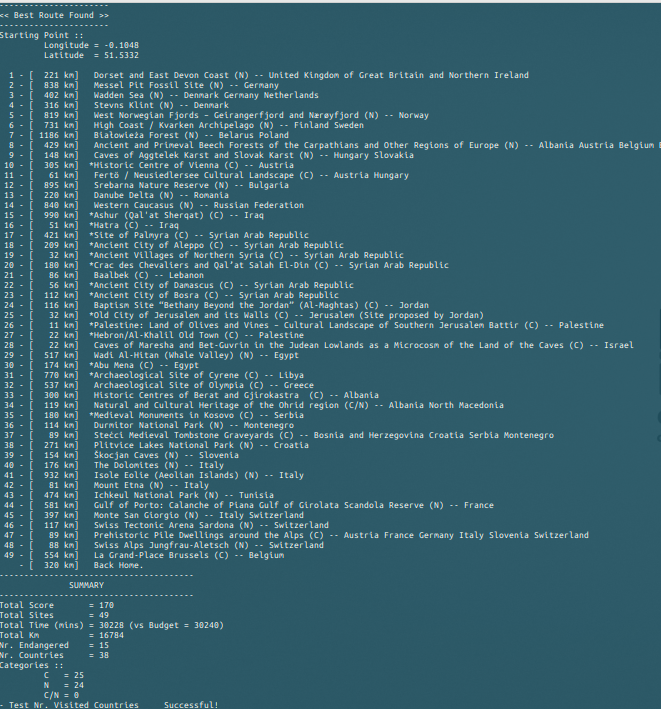
\includegraphics[scale=0.995]{example.png}
\caption{Example of a solution starting from London and visiting 49 sites, 38
countries.}
\label{fig:example}
\end{figure}

\section{UnitTests}

We designed tests for the following two categories:
\begin{itemize}
\item Tests for the evaluation functions: We thoroughtly tested that the
objective function value and the time limit are properly computed. The class
\texttt{TestFunctionsCorrectness} implements this type of tests.
\item Tests for the correctness of the final solution. We want to ensure that
the final solution complies with all the constraints of the model (including
the subtour constraints.) These tests, when successful, guarantee that the final
solution is actually feasible. The class \texttt{TestSolCorrectness} implements
this pool of tests.
\end{itemize}
In addition, beyond the use of unittests, the code uses standard
\texttt{assert()} clauses, which can be activated using the flag
\texttt{-ea} in compilation. These are aimed at ensuring that the update of the
objective function and of the travel time is properly carried out after each
move.

\section{Parameters of the Instance}

\begin{itemize}
\item The instance \texttt{whc-sites-2019.xl} has been transformed, using a
spreadsheet, into a \texttt{csv} file. The relevant portion of this file is found under
the folder \texttt{data}, file \texttt{unesco.csv}. This is the file that is
imported and used to compute the distances and the characteristics of each
site. Details about the Haversine transformation function are provided in the
code and its documentation.
\item Travel budget $B$. This is obtained assuming a travel duration of 3 weeks
(as stated in the specifications) and continuous travelling (since it is
mentioned that sleeping time can be assumed to occur during traveling.)
Therefore, we have:
\[
B = 21\times 24\times 60 = 3024~\text{minutes}
\]
\item Visit time: Specified as 6 hours per site, i.e., 360 minutes per site.

\end{itemize}








\end{document}
